	\begin{center}
		\Huge{\textbf{WARNING: .....Work in progress!}}
	\end{center}
\large
\label{Objective}
	
\subsection*{Principles}
This is an interactive document: It shall be modified on demand. \\
Each time, for each suggestion: mistakes, typos, a missing topics, something not clear, etc... 
\begin{center}
	E-mail \Letter: 
	\urlstyle{rm}
	\href{mailto:davidgueguen2000@yahoo.fr}{davidgueguen@mdl29.net}				
\end{center}
\begin{itemize}
	\item If you don't understand something this document is crap!	
	\item \lokiquote{sigmobile-2011-shannon}: link to pdf via choucroutage.com 
	\item \href{http://en.wikipedia.org}{Link}: link to wikipedia 
\end{itemize}

\subsection*{Objective}

\begin{itemize}	
\item The only reason for this document is to help in the understanding of an
	 attack/implementation. Tell if useful or not, pleaze, if there are thing missing.
	 
\item This document is far away from being enough to understand many modern attacks,
	for this reason it is mainly focus on implementation.	
\end{itemize}
As feasible as it is possible, was tried to make this document as precise and exact as possible 
on a mathematical point of view introducing systematically some required mathematical vocabulary. \\

To do :\\
*  give -anonymous- benchmark\\
*  give a precise estimation of the complexity, numerical examples\\
*  make system of references reliable  \\
*  refine the indexes of frequency\\
*  provide practical and theoretical ($\pm$) traces 

\subsection*{Thanx}
			\begin{figure}[h]
			\begin{center}
				
\includegraphics[scale=0.66]{images/logorfi.jpg}\\			\vspace{3mm}
	       		
\includegraphics[scale=4]{images/logoul.png}\\				\vspace{3mm}
	       		
\includegraphics[scale=0.66]{images/logoapplus.png}\\ 		\vspace{3mm}
	       		
\includegraphics[scale=0.75]{images/logochoucroutage.jpg}\\
			\end{center}
			\end{figure}


	\newpage
		\begin{figure}[h]
		\begin{center}
	       		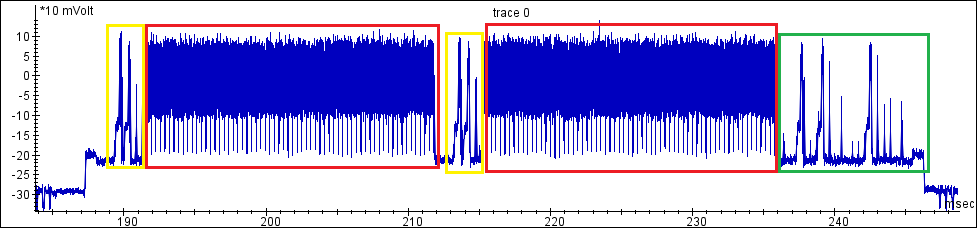
\includegraphics[width=18cm,height=5.5cm]{images/fullrsa.png}\\			\vspace{5mm}
	       		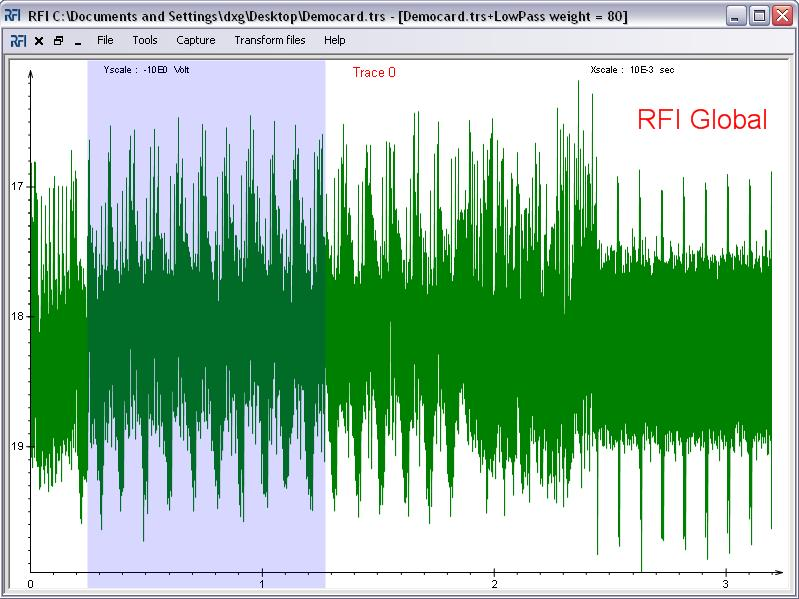
\includegraphics[width=18cm,height=5.5cm]{images/1.JPG}\\				\vspace{5mm}
	       		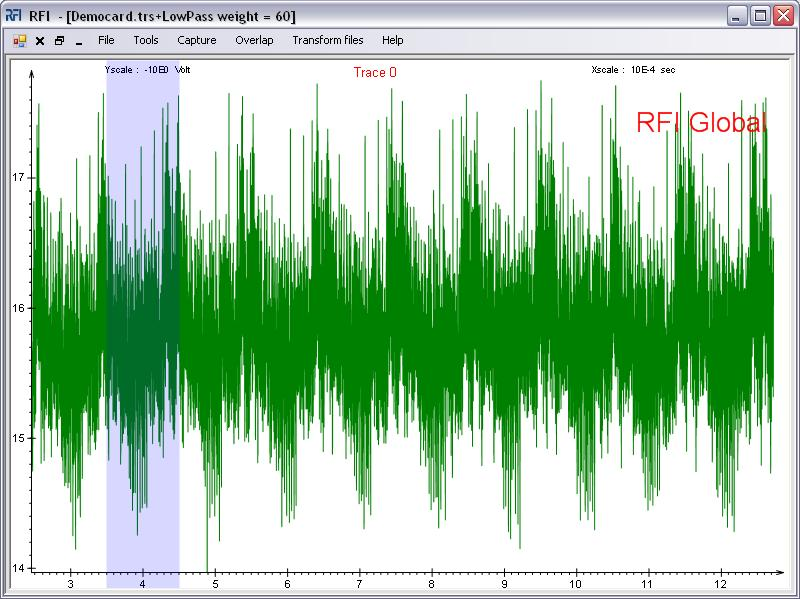
\includegraphics[width=18cm,height=5.5cm]{images/2.JPG}\\				\vspace{5mm}
	       		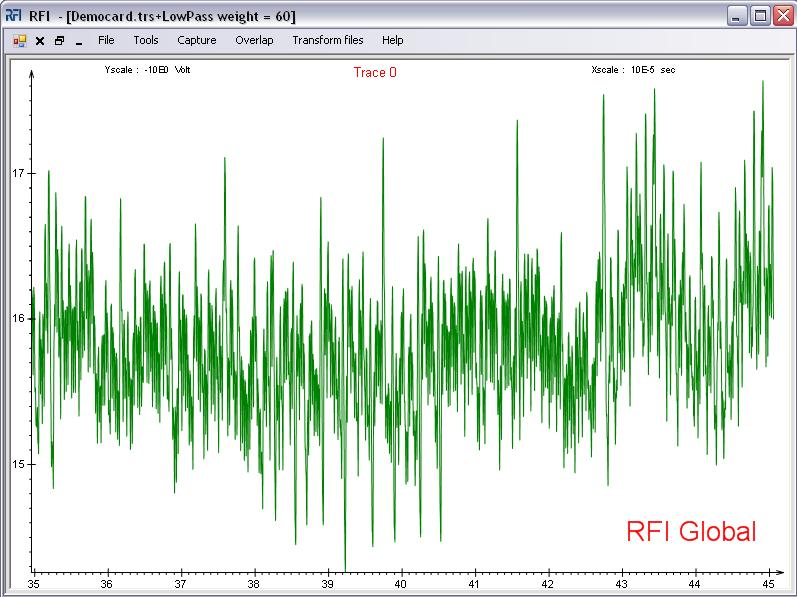
\includegraphics[width=18cm,height=5.5cm]{images/3.JPG}\\	
		\end{center}
		\end{figure}
	\newpage
	\tableofcontents
